% Nama Kelompok	: 	Kelompok 1 CPU
% Kelas		: 	D4 TI 1A
% Anggota	: 	1. Dezha Aidil Martha 1174025
% 			2. Habib Abdul Rasyid 1174002
% 			3. Muhammad Tomy Nur Maulidy 1174031
% 			4. Nico Ekklesia Sembiring 1174095
% 			5. Felix Setiawan Lase 1174026
% 			6. Damara Benedikta Siolemba 1174012
	


%Sejarah CPU
	\section{Sejarah CPU}
	\ref{CPU}
CPU adalah singkatan dari Central Processing Unit, CPU ini adalah bagian utama komputer yang berupa perangkat keras dan merupakan bagian paling penting dari komputer karena CPU ini berperan sebagai \"Otaknya\" Komputer. Fungsi CPU yang terdapat pada semua jenis komputer adalah untuk memproses data-data yang masukan lewat papan ketik dan tampilkan lewat layar monitor. Selain itu ada perkembangan CPU yang di bagi menjadi beberapa periode. Seperti yang tertulis pada artikel babmakalah \cite{babmakalah}


\begin{figure}[ht]
\centerline{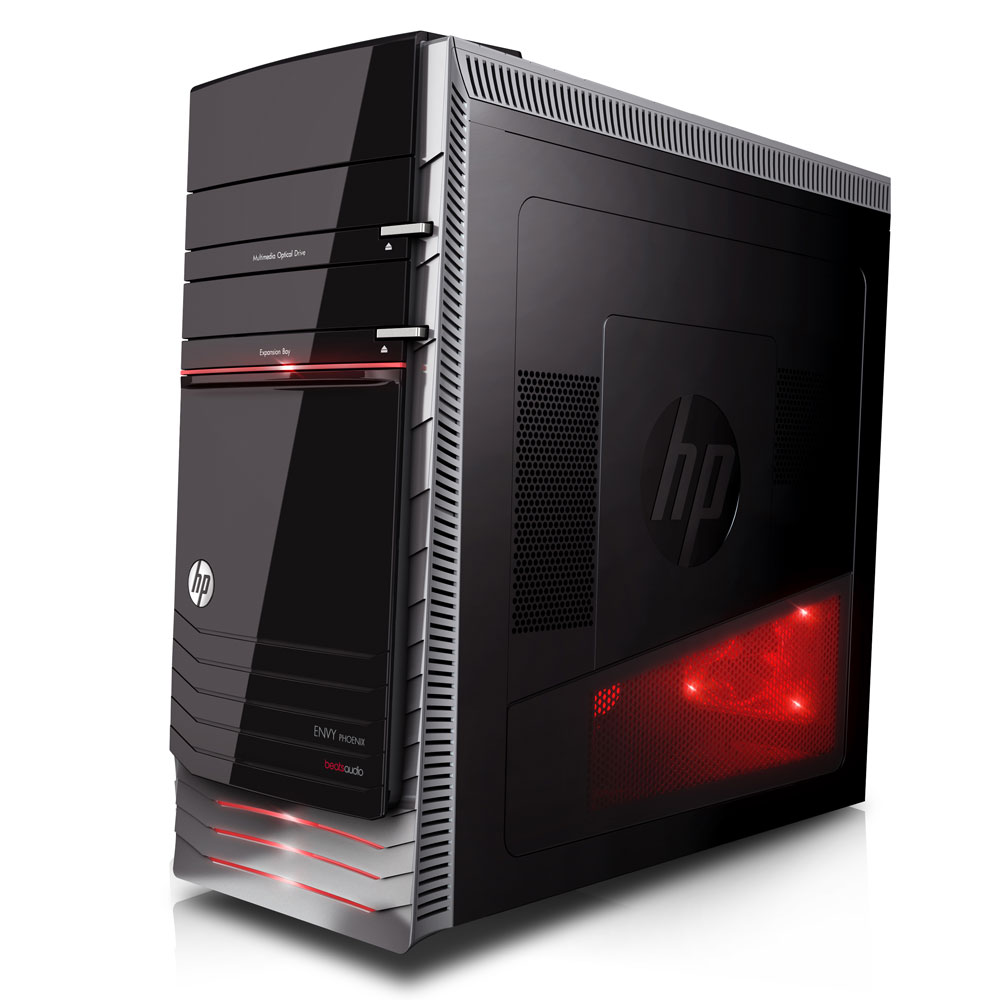
\includegraphics[width=1\textwidth]{figures/CPU.jpg}}
\caption{tampilan CPU}
\label{CPU}
\end{figure}

%CPU Generasi Pertama
	\section{Generasi ke pertama}
Pada Tahun 1945 IBM memproduksi CPU computer super besar yang dinamakan ENIAC ( Electrical Intregrator and Computer). CPU jenis ini dapat dikatakan sebagai moyangnya computer. ENIAC  terdiri dari 18.000 tabung yang kedap udara. Dalam pengoperasiannya diperlukan ruangan seluas 18x8 meter persegi.
Pada tahun 1951, CPU generasi pertama mengalami perkembangan dengan lahirnya computer ukuran besar pertama yang bernama EDVAC ( Electronic Discrete Variable Automatic Computer

%CPU Generasu Kedua
	\section{Generasi kedua}
 Tahun 1956 ditemukan transistor yang menjadi awal dari revolusi computer. Pada saat itu transistor menggantikan fungsi dari tube vakum pada televise,radio,dan computer. Yang menyebabkan ukuranya menjadi lebih kecil dari ukuran sebelumnya. Transitor juga mempunyai keunggulan lain yaitu mampu menghemat penggunaan listrik.
 Dan pada masa inilah bahasa pemograman mulai dikenal. Bahasa pemograman mempermudah banyak orang untuk menegrti computer dalam data. Dalam masa ini, computer banyak digunanakan untuk bisnis, karena mampu mengakses transaksi bisnis.

 %CPU Generasi Ketiga
 	\section{Generasi Ketiga}
 Pada tahun 1960-an Jack Kilby menemukan generasi ketiga oleh Intergrated Circuit, hal ini menjadi penanda terjadinya revolusi pada computer, khususnya pada cpu. IC mampu mencegah panas pada perangkat computer yang disebabkan oleh pemakaian transitor pada CPU.
 Meskiun transitor mengungguli tube vacum, tetapi menggunakan transitor menghasilkan panas yang cukup tinggi yang dapat merusak bagian bagian pada computer. 

 %CPU Generasi Keempat
 	\section{Generasi ke 4}
 Chip intel 4004 dibuat pada tahun 1971. Semua itu membawa banyak kemajuan yang cukup segnifikan bagi perkembangan CPU, pada saat itulah terjadi  penggabungan  berbagai komponen yang sebelumnya telah terpisah pada perangkat CPU tersebut, contoh dari komponen-komponen tersebut seperti : memori, bus dan prosesor , semua itu dapat disatukan hanya dalam satu perangkat Chip yang kecil.
	\subsection{Lanjutan Generasi Keempat}
 Komputer sekarang ukuran nya tidak lagi berukuran besarseperti dulu, sekarang lebih mini. pada awal 1970 mulaidiproduksi komputeruntuk semua orang, tidak hanya bagi yang pebisnis.
 Dulunya CPU pertama kali ada di dalam sebuah computer terpisahdengan monitor,namun penemuan laptop pada awal tahun 1990-an mengubah paradigm, bahwa sebuah computer harus berada pada suatu tempat tertentu.Apa lagi waktu itu kebutuhan terhadap laptop meningkat, maka penemuan laptop menjadi penemuan yang sangat menggembirakan. Saat itulah CPU mulai menyatu dengan monitor.


 %Sejarah Perkembangan microprocessor
 \section{Sejarah perkembangan microprocessor}
 	\ref{microprocessor}


 	\begin{figure}[ht]
\centerline{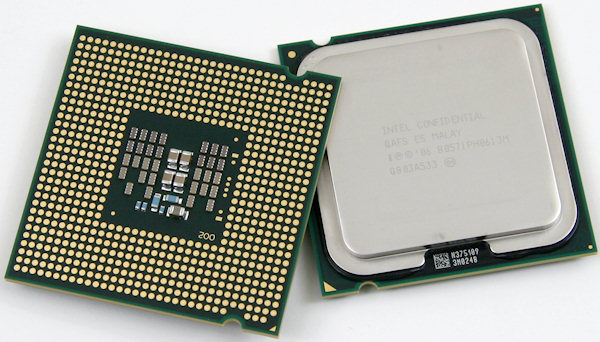
\includegraphics[width=1\textwidth]{figures/microprocessor}}
\caption{tampilan microprocessor}
\label{microprocessor}
\end{figure}
 		%Perkembangan Intel
 			\subsection{perkembangan tahun 1971:4004 microprocessor}
 	Pada tahun 1971 munculah microprocessor pertama Intel, microprocessor bertype 4004 ini pertama kali digunakan pada mesin kalkulator Busicom. dengan penemuan ini membukakan jalan untuk mengembangkan dalam pembuatan pada benda mati.
 			\subsubsection{Perkembangan pada tahun 1972:8008 Microprocessor}
 	pada tahun 1972 keluarlah microprocessor 8008 yang memiliki tenaga 2 kali lipat dari versi sebelumnya yaitu 4004.

 	
 			\subsubsection{perkembangan tahun 1974:8080 microprocessor}
 	micropocessor 8080 menjadi otak dari sebuah komputer yang bernama altair, saat itu sudah terjadi sepuluh ribu penjualan dalam satu bulan
 			\subsubsection{perkembangan tahun 1978:8086-8088 micropocessor}
 	pada tahun 1978 terdapat sebuah penjualan penting didalam devisi komputer penjualan tersebut terjadi pada produk-produk komputer pribadi buatan IBM yang menggunakan processor 8088 yang berhasil mendongkrak nama intel dalam penjualan produk


 			\subsubsection{1982: 286 Microprocessor}
 	Intel mengeluarkan processor seri 286 atau yang lebih dikenal dengan kode 80286, 80206 adalah sebuah processor pertama yang dapat mengenali software yang digunakan pada processor sebelumnya.
 			\subsubsection{1985: Intel386™ Microprocessor}
 	Setelah Intel 286, Intel meluncurkan processor yang memiliki 275.000 transistor yang tertanam pada processor itu, yang jika dibandingkan dengan seri 4004 memiliki 100x lipat lebih banyak transistor.

 			\subsubsection{1989 : Intel486™ DX CPU Microprocessor}
 	Pada tahun 1989 untuk yang pertama kali  ditemukan proccesor yang dapat mempermudah berbagai aplikasi yang sebelumnya harus mengetikkan command command dan pada Intel486 CPU Microprocessor hanya dengan sebuah klik saja. Pada processor ini juga mempunyai fungsi komplek matematika yang mempunyai fungsi untuk memperkecil beban processor.
 			\subsubsection {1993 : Intel® Pentium® Processor}
 	Pada tahun 1993 diciptakan processor generasi baru yang dapat menangani berbagai jenis data seperti bunyi, suara, foto, dan tulis tangan.


 			\subsubsection{Intel Pentium Pro Processor (1995)}
 	Intel Pentium pro dirancang untuk digunakan pada operasi server dan workstation, yang diciptakan untuk memproses data secara cepat, Processor ini memiliki 5,5 juta traansistor yang tertanam
 			\subsubsection{Intel Pentium II Processor (1997)}	
 	Processor Pentium II ini adalah processosr yang menggabungkan Intel MMX yang dirancang secara khusus untuk mengelolah data video,audio, dan grafik secara efisien. Terdapat sekitar 7.5 juta transistor sehingga dengan processor ini pengguna PC dapat mengelolah berbagai data yang ada di dalamnya dan menggunakan internet dengan lebih baik lagi.


 			\subsubsection{Perkembangan tahun 1998: Intel Pentium II Xeon Processor}
 	Processor jenis ini dibuat dengan tujuan untuk memenuhi kebutuhan pada aplikasi server. Saat itu perusahaan Intel memiliki strategi dengan memghadirkan processor unik untuk kebutuhan pasar
 			\subsubsection{Perkembangan tahun 1999 : Intel Celeron Processor}
 	Processor jenis ini merupakan jenis proessor yang dihadirkan sebagai processor yang diperuntukkan kepada pengguna yang tidak membutuhkan processor yang lebih cepat dengan harga yang tidak terlalu besar. Processor ini memiliki kesamaan bentuk dan fromfactor dengan jenis intel Pentium. Tetapi dengan sedikit perbedaan pada kinerja, instruksi, dan ukuran cache nya


 			\subsubsection{1999 : Intel® Pentium® III Processor}
 	Pada tahun 1999 dikembangkan 3 processor, yaitu salah satunya adalah Intel Pentium 3. Intel Pentium III diberi fitur tambahan 70 instruksi baru yang sangat membantu dalam memperkaya kemampuan dalam pencitraan tingkat tinggi, audio streaming, tiga dimensi, dan aplikasi aplikasi video serta pengenalan suara. 
 			\subsubsection{1999 : Intel® Pentium® III Xeon® Processor}
 	Processor terkahir yang dikembangkan pada tahun 1999 adalah Intel Pentium 3 Xeon. Dengan dirilisnya Intel Pentium 3 Xeon, Intel merambah pasaran server dan workstation. Processor ini mempunyai 70 SIMD, processor ini juga dirancang dapat dipadukan dengan processor lain yang sejenis. Bukan cuman itu keunggulan Intel Pentium 3 Xeon, processor ini juga dapat meningkatkan kinerja dalam pengolahan informasi dari system bus menuju processor, dan processor ni juga dapat meningkatakan performa secara signifikan.


			\subsubsection{2000 : intel pentium 4 processor}
 	processor pentium 4 adalah produk intel yang dirilis tahun 2000 dengan kecepatan prosesnya mampu mencapai 3.06GHz. processor ini mempunyai kecepatan 1.5GHz dengan formfactor pin 423, setelah itu intel merubah formfactor processor Intel Pentium 4 menjadi pin 478 yang dimulai dari processor intel pentium 4 dengan kecepatan 1.3GHz sampai yang terbaru yang saat ini mampu menembus hingga kecepatan 3.4GHz.


			\subsubsection{2001 intel xeon processor}
 	Processor Intel Pentium 4 Xeon adalah processor Intel Pentium 4 yang bertujuan mampu berperan dalam computer server. Processor ini memiliki jumlah pin yang lebih banyak dari pada processor Intel Pentium 4 serta memiliki memory L2 cache yang lebih besar pula.
 			\subsubsection{2001 Intel itanium processor}
 	processor Intel Itanium adalah processor yang dirilis dengan basis 64bit, processor tersebut ditujukan untuk pemakai server dan workstation serta para pemakai tertentu. Processor ini di ciptakan dengan struktur dan disain yang benar-benar berbeda dengan sebelumnya. Disain dan teknologi processor ini didasarkan pada \"Intels Explicity Parallel Instruction Computing\" atau bisa disebut EPIC.


 			\subsubsection{Perkembangan tahun 2002 : Intel Itanium 2 Processor }
 	Pada tahun 2002 diluncurkan juga Intel Itanium 2 sebagai generasi kedua dari processor jenis Itanium. Hadirnya processor ini memberikan dampak positif bagi penggunanya karena telah meringankan masalah dari kinerja processor generasi sebelumnya.
 			\subsubsection{Perkembangan tahun 2003 : Intel Pentium M processor}
 	Intel Pentium M Processor diluncurkan oleh Intel pada tahun 2003. Processor jenis ini menggunakan Chipset 855 dan Intel PRO/Wirelless 2100 sebagai komponen nya. Intel Pentium M Processor juga sering disebut dengan Intel Centrino
 			\subsubsection{Perkembangan tahun 2004 : Intel Pentium M 735/745/755 Processor}
 	Processor jenis ini diciptakan sebagai kelanjutan dari generasi Pentium sebelumnya. Processor ini diciptakan dengan menambahkan fitur baru 2Mb L2 Cache 400Mhz sistem bus.


 			\subsection{Intel Pentium 4 Extreme Edition 3.73GHz}
 	Pada tahu 2005 dikembangkan Intel Pentium 4 Extreme Edition, processor ini diperuntukkan untuk pengguna komputer yang menginginkan sesuatu yang lebih dari yang ada didalam komputer miliknya. Pada processor ini menggunakan konfigurasi  3.73GHz frequency, 2MB L2 cache, EM64T, 1.066GHz FSB, dan menggunakan Hyper Threading. Dan beberapa bulan kemudian muncul Intel Pentium D 820/830/840. Processor ini berbasis 64 bit dan memiliki konfigurasi 1MB L2 cache pada tiap core

	
			\subsubsection{2006: Intel Core 2 Quad Q6600}
 	Bagi orang orang yang ingin memiliki kekuatan yang lebih lebih pada komputernya, pada tahun 2006 diciptakan Intel Core 2 Quad Q6600 yang memiliki 2 buah core dengan konfigurasi processor 2.4 GHz dengan 8 Mb L2 Cache, 1.06 GHz Front Size bus dan therma l design power atau TDP.
 			\subsubsection{2006: Intel Quad-core Xeon X3210/X3220}
 	Processor Quad-core Xeon X3210/X3220 memiliki 2 buah core dengan setiap core dikonfigurasi processor 2.13Ghz dan 2.4Ghz, dengan ukuran 8Mb L2 Chace (Bisa diupgrade 4Mb untuk setiap core) 1.06Ghz untuk Front-side bus, dan TDP.


 			\subsubsection{2008 : Intel i7}
 	Pada tahun 2008 diciptakan processor intel i7 yang mempunyai nama kode \"Nehalem\". Pada awal dibuat pelanggan setia intel sulit mengingat namanya karena dirubah menjadi nehalem. Intel i7 mempunyai beberapa keunggulan, diantaranya:
 		1. Performa dan efisisen lebih tinggi dalam pengguaan energi
 		2. Fungsi Front Side Bus diganti Quick Path Interface
 		3. Processor ini memiliki memory controll
 		4. Intel i7 didukung Three Channel Memory
 		5. Processor ini menggunakan single die device:memory controller, core (inti processor), dan cache berada dalam satu die.
 		6. I7 didukung tipe socket baru yaitu Socket B (Socket LGA 1366)

 %Perkembangan AMD
 		\section(AMD)
 		\ref{AMD}


\begin{figure}[ht]
\centerline{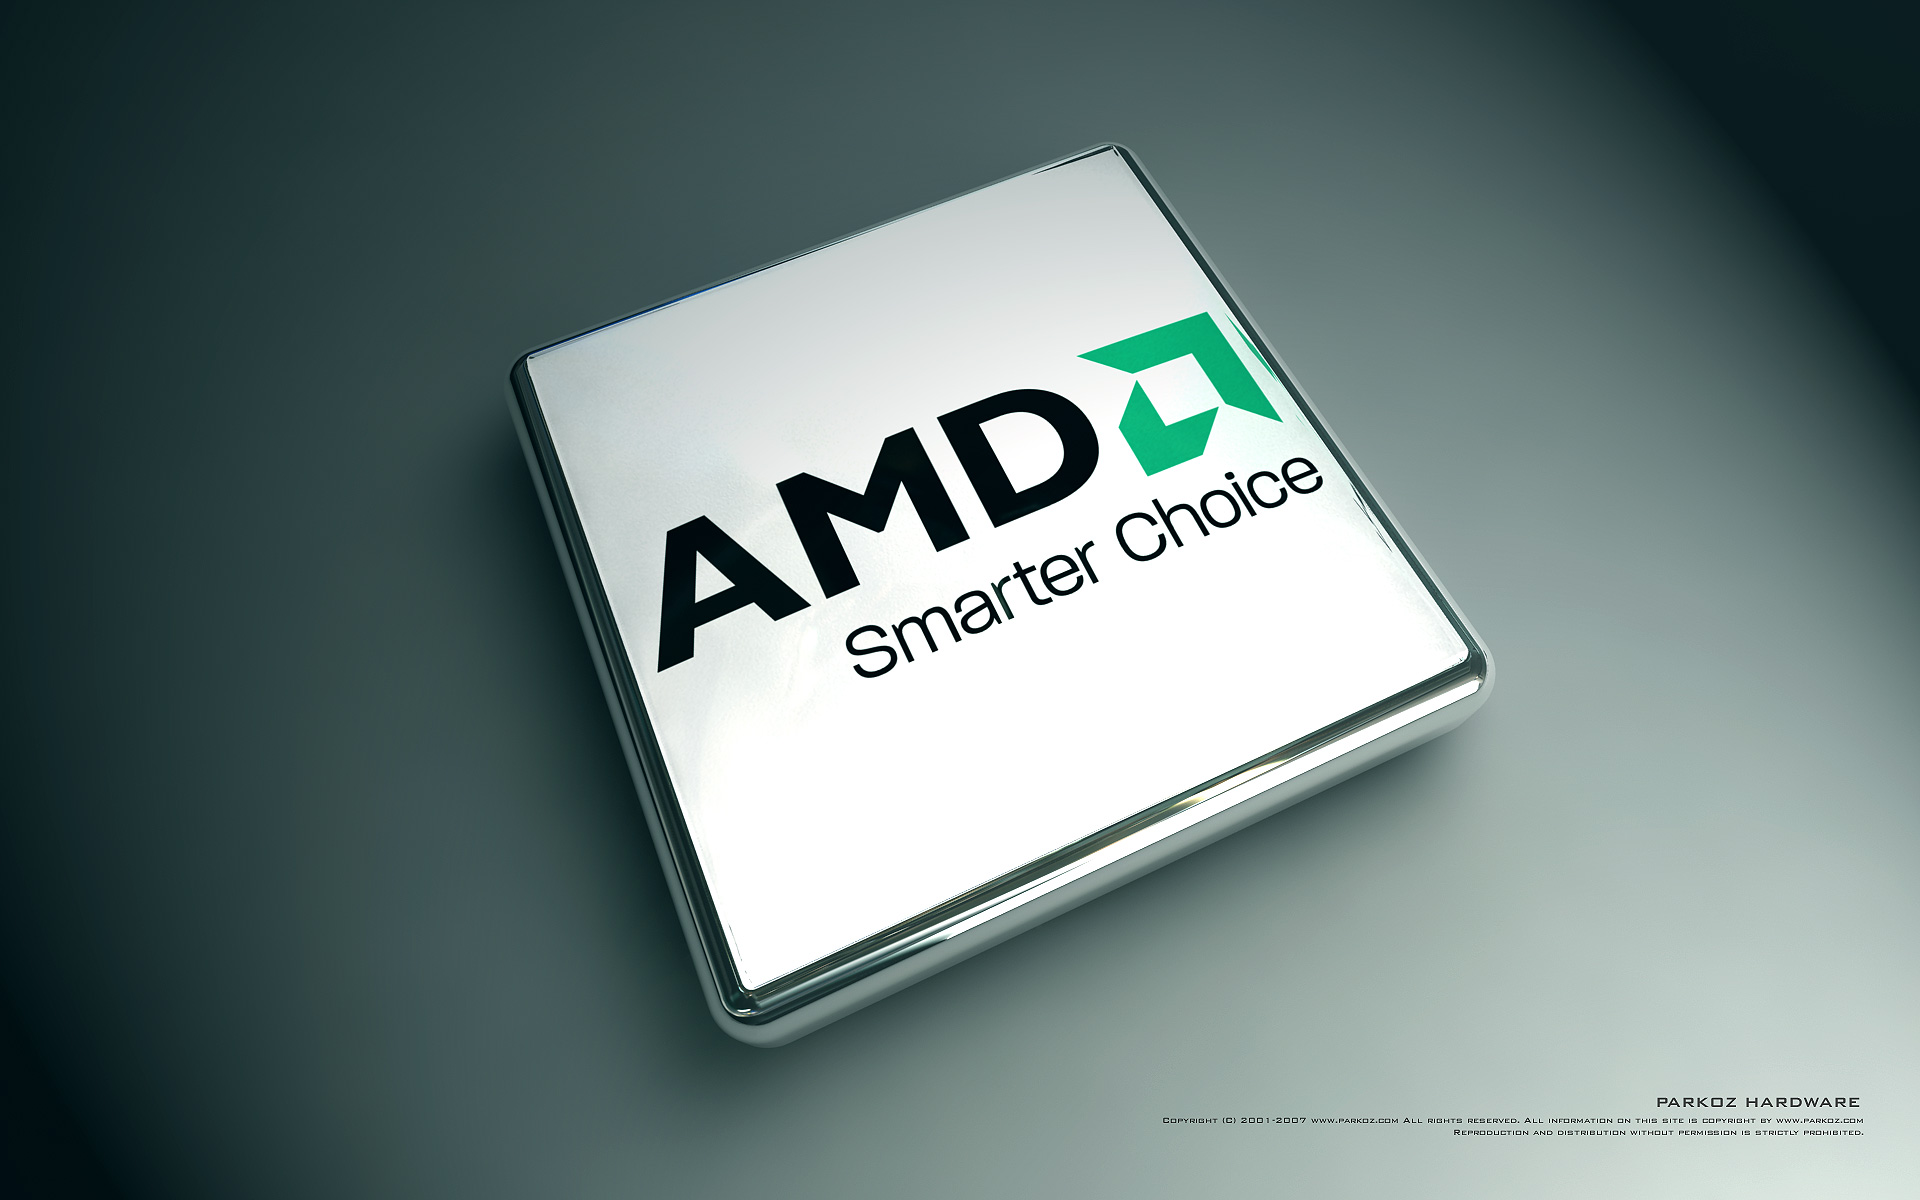
\includegraphics[width=1\textwidth]{figures/AMD.JPG}}
\caption{tampilan AMD}
\label{AMD}
\end{figure}
 			\subsection{ AMD K5 }
 	AMD K5 dibuat pada awalnya agar dapat bekerja dengan semua motherboard yang mendukung intel tersebut. Jadi motherboaed yang mendukung intel tersebut akan mendukung pula AMD K5. Pada saat itu tidak semua motherboard langsung dapat mengenali AMD dan harus melakukan upgrade BIOS untuk dapat mengenali AMD.
 			\subsection{ AMD K6 }
 	processor AMD K6 adalah processor generasi ke-6 memiliki performa yang tinggi dan dapat diinstalasi motherboard yang mendukung intel pentium. AMD K6 memiliki beberapa model diantaranya : AMD K6, AMD K6-2, AMD K6-III.


			\subsubsection{AMD Duron}
 	Processor series AMD ke 3 yaitu AMD Duron merupakan salah satu versi processor murah yang terkenal pada tahun 2008, pada awalnya ini memiliki kode nama Spitfire yang dibuat berdasarkan Thunderbird Core. AMD Duron merupakan versi ringkasan dari AMD Atheon, ia mempunyai semua arsitektur yang dimiliki oleh AMD  Athlon
 			\subsubsection{AMD Athlon}
 	AMD Athlon merupakan seri pengganti dari seri AMD sebelumnya yang bernama AMD Ko. Tujuan AMD mengeluarkan seri ini untuk menggeser Perusahaan Microprocessor Intel yang merupakan pemimpin pasar industri microprocessor. Dalam menjalankan tujuannya tersebut, AMD menambahkan beberapa fitur tambahan, yakni dua instruksi untuk 3D Now dan dua instruksi untuk MMX yang terdapat dalam pipe floating point. Jenis microprocessor ini telah berhasil mengungguli Intel Pentium III Coppermine.


 			\subsubsection{AMD Athlon 64}
 	Processor AMD athlon 64 memiliki 3 varian socket yang berbeda, yaitu 754,939, dan 940. pada socket 754 memiliki kontroler memori yang mendukung penggunaan memori DDR kanal tunggal. socket 939 memiliki Kontroler memori yang mendukung memori kanal ganda. AMD Athlon ini merupakan processor pertama yang kompatibel terhadap komputer dengan basis 64bit.  teknologi AMD 64 yang terdapat pada processor tersebut mampu berjalan dalam operasi sistem 32bit maupun 64bit.


 			\subsubsection {AMD Sempron}
 	processor tersebut merupakan jajaran processor yang di kenalkan oleh AMD pada tahun 2004, processor ini merupakan processor pengganti dari processopr AMD Duron.Pada beberapa seri AMD Sempron fitur yang dapat digunakan hanyalah fitur 32bit sedangkan fitur 64bit dinonaktifkan.
 			\subsubsection {Versi AMD Sempron}
 	 1.AMD Sepron soket A merupakan varian yang dibuat berdasarkan pada processor AMD Althon Thoroughbred. Karena pada saat tersebut AMD telah meluncurkan processor baru untuk pasar High-End AMD Althon 64.
 	 2.AMD Sempron Soket 754 merupakan processor Sempron yang dibuat di atas arsitektur AMD 64 yang bertujuan untuk meningkatkan kinerja yang telah dimiliki.


			\subsubsection{AMD 64 X2 Dual Core}
 	Processor ini bertujuan untuk mengimbangi apa yang telah dikembangkan Intel dengan Processor Core Duo. Processor ini tetap memiliki basis 64 bit,dan ini ditujukan bagi pengguna media digital yang intensif
 	Dari sisi fiturnya processor ini dibekali dengan HyperTransport yang dapat meningkatkan kinerja system secara keseluruhan dengan menghapus bottlenecks pada level input output, meningkatkan badwith,dan mengurangi latency system. Pendekatan nya adalah kontrol memori DDR yang sepenuhnya terintegrasi sehingga dapat membaty mempercepat akses ke memori. Hasilnya adalah bias menikati loading yang lebih cepat pada aplikasi.


 			\subsubsection{AMD Opteron}
	AMD Opteron dirilis pada musim semi, processor ini dirilis untuk pasar server dan workstation. AMD Opteron memiliki beberapa fitur, yaitu:
		1. Chache tingkat 1 sebesar 128kb
		2. Chache tingkat 2 sebesar 1024kb
		3. Kecepatan mulai dari 1400MHz hingga 3000MHz
		4. Processor ini dilengkapi 3 buah link Hyper Transport yang memiliki kecepatan 3200 Mbit/s
		5. Sanggup mengakses memori fisik hingga 1 TB 


			

			\subsubsection{Kemampuan Processor Intel dan AMD}
 	Melihat dari tahun ke tahun seiring perkembangan processor yang semakin pesat baik dari segi kapasitas maupun kemampuan. perkembangan processor sangat berpengaruh untuk membantu pengembangan software yang mana perkembangan software juga harus diimbangi dan terus ditingkatkan kemampuannya. para produsen penghasil processor terus mengembangkan kinerja processor mereka. processor yang saat ini menguasai pemasaran dalam bidang teknologi yaitu adalah Intel dan AMD kedua processor ini sudah diakui kemampuannya, kedua processor ini mampu bekerja dengan akses yang cepat menghasilkan kualitas grafis yang sangat baik dan cocok sekali bagi para pengembang program.\cite{irwansyah2014pengantar} 




 %Sekilas tentang CPU
 	\section{Sekilas tentang CPU}
 	Sejak tahun 1960an, Istilah penamaan processor sentral ini sudah dipakai dalam Industri komputer. seiring dengan perubahan zaman yang semakin pesat terutama dalam bidang teknologi mulai dari bentuk sampai desain mengalami perkembangan yang signifikan, namun Operasi dari CPU tetap sama hingga sekarang. bahkan saat ini sebuah komputer dapat memiliki lebih dari CPU. cara ini biasa disebut multiprocessor, beberapa sirkuit terpadu (intergrated Circuit) dapat berisi beberapa CPU dalam satu chip.
 
 	Dalam model komputasi terdistribusi, masalah ini diselesaikan oleh satu set saling didistribusikan prosesor. Adapun kegunaan dari CPU ini adalah sebagai otak atau inti dari semua proses yang dijalankan oleh komputer.



 %Bagian-bagian CPU
 	\section{Bagian bagian CPU}
 	Dalam penulisan makalah mengenai CPU harus dicantumkan bagian bagian CPUnya.dan salah satu bagian nya adalah sebagai berikut
 			\subsubsection{Motherboard (Papan Sirkuit)}
 		Motherboard ini biasa disebut dengan papan sirkut komputer karna merupakan tempat bagi semua komponen yang terhubung .papan sirkut ini berisi mikroprocessor, komponen penting seperti komputasi,memiliki berbagai jenis chip memori,port mouse,keyboard,dan meninjau sirkuit kontrol, dan logika chip yang mengontrol berbagai bagian fungsi komputer tersebut.memiliki banyak komponen kunci dari komputer mungkin motherboard dapat meningkatkan kecepatan dan pengoperasian komputer tersebut.


 			\subsubsection{ALU}
 		Arithmetic and Logical Unit atau ALU adalah salah satu bagian dari CPU yang memiliki tugas untuk memproses data secara logika dan data-data yang membutuhkan hitungan angka yang sesuai dengan instruksi. ALU merupakan sekumpulan register-register yang dapat menyimpan segala informasi yang diperlukan.
 			\subsubsection{Register Source}
 		Register Source adalah sekumpulan alat-alat yang dapat menyimpan data dan mempunyai akses dengan kecepatan yang tinggi saat instruksi sedang berlangsung.


 			\subsubsection{CD ROM}
 		Compact Disk Read Only Memori atau yang sering disebut dengan CD ROM. Dengan menggunakan laser optikal teknologi terdapat pada disk nya, CD ROM dapat membaca informasi didalam nya, Namun
 		tidak dapat menulis informasi atau data didalam CD tersebut. Tapi saat ini dengan perkembangan teknologi hal itu sudah bisa dilakukan.
 			\subsubsection{VGA Card}
 		VGA/VGA Card (Kartu Grafis) adalah sebuah kartu yang terhubung ke motherboard/papan induk. Kartu ini berfungsi sebagai media visualisasi antara perangkat dengan pengguna.


 			\subsubsection{Hard Disk}
 		Hard disk adalah perangkat keras yang berfungsi sebagai media penyimpanan utama pada komputer. Dapat juga disebut dengan hard drive. Hard disk biasanya menggunakan disk yang  terbuat dari kaca atau aluminium. Dalam perkembangannya, hard disk dirancang semakin tipis dan kecil, namun dengan daya penyimpanan yang cukup besar. Ukuran penyimpanan terbesar hard disk yang ada pada saat ini mencapai 3 Tera Byte yang memiliki ukuran sebesar 3,5 inci
 			\subsubsection{Floppy Disk}
 		Floppy disk biasa disebut dengan disket. Floppy disk merupakan media penyimpaan yang tipis dan fleksibel dan dibungkus atau disegel dengan plastic yang berbentuk persegi atau persegi panjang. Dalam penggunaannya, Floppy disk dapat dilepas dan dipasang kembali ke computer. Namaun sejak tahun 2010, Floppy disk sudah jarang digunakan karena sudah jarang mother board computer diproduksi dengan menggunakan media floppy drive.



 			\subsubsection{Cara kerja CPU}
 		Banyak orang yang menyebutkan otak komputer adalah CPU. Hal ini didasari karena CPU menjalankan semua perintah dan program. CPU dapat membandingkan hal lainnya yang brsifat komputasi dan CPU juga dapat mengitung data berupa logika dan aritmatika. Cara kerja CPU adalah pada saat si pengguna meberikan arahan maka arahan tersebut di masukkan ke dalam processor melalui input penyimpanan. Perintah atau instruksi tersebut disimpan oleh kontrol unit di program penyimpanan. Apabila perintah berupa data maka data disimpan di penyimpanan kerja. 



 			\subsubsection{Fungsi CPU}
 		CPU memiliki fungsi utama, yakni menjalankan program yang tersimpan dalam memori utama dengan cara mengambil instruksi, melakukan pengujian  instruksi, dan melakukan pengeksekusian sesuai alur perintah yang diberikan. Dalam proses pengeksekusian program, terdapat pengolahan instruksi yang terdiri dari dua langkah. Yakni operasi pembacaan (Fetch) dan operasi pelaksanaan (Execute). Saat program sedang dieksekusi, data dialirkan dari RAM kedalam unit yang menghubungkan antara CPU dengan RAM yang disebut dengan bus.